\documentclass{mpaper}
\usepackage{bm}
\usepackage{bbm}
\usepackage{mathtools}
\usepackage[UKenglish]{babel}
\usepackage[UKenglish]{isodate}

\newtheorem{theorem}{Theorem}[section]
\newtheorem{proposition}[theorem]{Proposition}
\newtheorem{lemma}[theorem]{Lemma}
\newtheorem{definition}[theorem]{Definition}
\newtheorem{remark}[theorem]{Remark}

\DeclareMathOperator{\diag}{diag}
\DeclareMathOperator{\adj}{adj}
\DeclareMathOperator{\tr}{tr}
\DeclareMathOperator*{\argmax}{arg\,max}

\DeclarePairedDelimiterX{\infdivx}[2]{(}{)}{%
  #1\;\delimsize\|\;#2%
}
\newcommand{\DKL}{D_{\mathrm{KL}}\infdivx}
\newcommand{\V}{V_{\mathbf{r}}}
\newcommand{\dx}{\,d\mathbf{r}\,d\mathbf{u}}
\newcommand{\vbound}{\frac{\rinf + \log|\mathcal{A}|}{1 - \gamma}}
\newcommand{\rinf}{\lVert \mathbf{r} \rVert_\infty}

\newcommand{\f}{f(\mathbf{r}, \mathbf{u}, t)}
\newcommand{\fn}{f_n(\mathbf{r}, \mathbf{u})}
\newcommand{\ftn}{f(\mathbf{r}, \mathbf{u}, t_n)}
\newcommand{\g}{g(\mathbf{r}, \mathbf{u})}

\newcommand{\Kuu}{\mathbf{K}_{\mathbf{u},\mathbf{u}}}
\newcommand{\Krr}{\mathbf{K}_{\mathbf{r},\mathbf{r}}}
\newcommand{\Kru}{\mathbf{K}_{\mathbf{r},\mathbf{u}}}
\newcommand{\Luu}{\mathbf{L}_{\mathbf{u},\mathbf{u}}}

\newcommand{\pfull}{p(\mathcal{D}, \mathbf{u}, \mathbf{r})}
\newcommand{\approximation}{q(\mathbf{u}, \mathbf{r})}
\newcommand{\posterior}{p(\mathbf{u}, \mathbf{r} \mid \mathcal{D})}

\newcommand{\dm}{\frac{\partial}{\partial\bm\mu}}
\newcommand{\dB}{\frac{\partial}{\partial\mathbf{B}}}
\newcommand{\dl}{\frac{\partial}{\partial \lambda_i}}
\newcommand{\dlj}{\frac{\partial}{\partial \lambda_j}}
\newcommand{\dt}{\frac{\partial}{\partial t}}
\newcommand{\df}{\left.\frac{\partial f}{\partial t}\right|_{(\mathbf{r},
    \mathbf{u}, t)}}

\begin{document} % 14 pages

\title{Variational Inference for Inverse Reinforcement Learning with Gaussian Processes}
\author{Paulius Dilkas}
\matricnum{2146879}
\maketitle

\begin{abstract}
\end{abstract}

% TODO: add info from slides/handout
\section{Introduction}
% problem description/statement

% TODO: will need to rewrite this to avoid plagiarism
Inverse reinforcement learning (IRL)---a problem proposed by Russell in
1998 \cite{DBLP:conf/colt/Russell98}---asks us to find a reward function for a
Markov decision process (MDP) that best explains a set of given demonstrations.
IRL is important because reward functions can be hard to define manually
\cite{DBLP:conf/icml/PieterN04,DBLP:journals/corr/abs-1806-06877}, and rewards
are not entirely specific to a given environment, allowing one to reuse the same
reward structure in previously unseen environments
\cite{DBLP:journals/corr/abs-1806-06877,DBLP:conf/uai/JinDAS17,DBLP:conf/nips/LevinePK11}.
Moreover, IRL has seen a wide array of applications in autonomous vehicle
control \cite{DBLP:journals/ijsr/KimP16,DBLP:journals/ijrr/KretzschmarSSB16} and
learning to predict another agent's behaviour
\cite{DBLP:journals/ai/BogertD18,DBLP:conf/aaai/VogelRGR12,ziebart2008maximum,DBLP:conf/huc/ZiebartMDB08,DBLP:conf/iros/ZiebartRGMPBHDS09}.
Most approaches in the literature (see Section \ref{sec:background}) make a
convenient yet unjustified assumption that the reward function can be expressed
as a linear combination of features. One proven way to abandon this assumption
is by representing the reward function as a Gaussian process (GP)
\cite{DBLP:conf/uai/JinDAS17,DBLP:conf/nips/LevinePK11,DBLP:journals/corr/abs-1208-2112}.
The original approach used maximum likelihood estimation
\cite{DBLP:conf/nips/LevinePK11}, while the goal of this project is to use
variational inference (VI) instead, which learns approximate posterior
probability distributions instead of point estimates. This approach can prove
useful in three major ways:
\begin{enumerate}
\item Modelling full posterior distributions for various parameters can result
  in more precise reward predictions, as the model simply holds more
  information.
\item Having variance estimates for rewards can direct our choice in what data
  should be collected next.
\item An approximate Bayesian treatment of many parameters in the model guards
  against overfitting \cite{DBLP:conf/uai/JinDAS17}.
\end{enumerate}

\subsection{Statement of the Problem}

\begin{definition}[MDP]
  A \emph{Markov decision process} is a set $\mathcal{M} = \{ \mathcal{S},
  \mathcal{A}, \mathcal{T}, \gamma, r \}$, where $\mathcal{S}$ and
  $\mathcal{A}$ are sets of states and actions, respectively; $\mathcal{T} :
  \mathcal{S} \times \mathcal{A} \times \mathcal{S} \to [0, 1]$ is a function
  defined so that $\mathcal{T}(s, a, s')$ is the probability of moving to state $s'$
  after taking action $a$ in state $s$; $\gamma \in [0, 1)$ is the discount
  factor (with higher $\gamma$ values, it makes little difference whether a
  reward is received now or later, while with lower $\gamma$ values the future
  becomes gradually less and less important); and $r : \mathcal{S} \to
  \mathbb{R}$ is the reward function.
\end{definition}

In \emph{inverse reinforcement learning}, one is presented with an MDP without a
reward function $\mathcal{M} \setminus \{ r \}$ and a set of expert
demonstrations $\mathcal{D} = \{ \zeta_i \}_{i=1}^N$, where each demonstration
$\zeta_i = \{ (s_{i,0}, a_{i,0}), \dots, (s_{i,T}, a_{i,T}) \}$ is a multiset of
state-action pairs representing the actions taken by the expert during a
particular recorded session. Each state is also characterised by a number of
features. The goal of IRL is then to find $r$ such that the optimal policy under
$r$
\[ \pi^* = \argmax_\pi \mathbb{E}\left[ \left. \sum_{t=0}^\infty \gamma^t r(s_t)
    \right| \pi \right] \]
matches the actions in $\mathcal{D}$.

Following previous work on GP IRL
\cite{DBLP:conf/nips/LevinePK11,DBLP:conf/uai/JinDAS17}, we use a maximum
entropy IRL model \cite{ziebart2008maximum}, under which we have that
\[ P(a | s) \propto \exp(Q_{\mathbf{r}}(s, a)), \]
where
\[
  Q_{\mathbf{r}}(s, a) = r(s) + \gamma\sum_{s' \in \mathcal{S}}
  \mathcal{T}(s, a, s')\V(s'),
\]
and $\V : \mathcal{S} \to \mathbb{R}$ is an MDP \emph{value function}, which
can be obtained by repeatedly applying the 'soft' version of the Bellman backup
operator until convergence:
\cite{DBLP:conf/nips/LevinePK11,supplementary_material}
\begin{equation} \label{eq:update_rule}
  \V(s) \coloneqq \log \sum_{a \in \mathcal{A}} \exp\left( r(s) + \gamma\sum_{s'
      \in \mathcal{S}} \mathcal{T}(s, a, s')\V(s') \right).
\end{equation}
The likelihood of the data can then be expressed as
\cite{DBLP:conf/uai/JinDAS17,DBLP:conf/nips/LevinePK11}
\begin{equation} \label{pDr}
  \begin{split}
    p(\mathcal{D} | r) &= \prod_{i=1}^N \prod_{t=1}^T p(a_{i,t} | s_{i,t}) \\
    &= \exp\left( \sum_{i=1}^N \sum_{t=1}^T Q_{\mathbf{r}}(s_{i,t}, a_{i,t}) - \V(s_{i,t}) \right).
  \end{split}
\end{equation}
However, a reward function learned by maximising this likelihood is not
transferable to new situations
\cite{DBLP:conf/uai/JinDAS17,DBLP:conf/nips/LevinePK11}. One needs to model the
reward structure in a way that would allow reward predictions for previously
unseen states.

One way to model rewards without assumptions of linearity is with a
\emph{Gaussian process} (GP). A GP is a collection of random variables, any
finite combination of which has a joint Gaussian distribution
\cite{DBLP:books/lib/RasmussenW06}. We write $r \sim \mathcal{GP}(0,
k)$ to say that $r$ is a GP with mean $0$ and covariance function
$k$, which uses a vector of hyperparameters $\bm\lambda$.
Covariance functions take two state feature vectors as input and quantify how
similar the two states are, in a sense that we would expect them to have similar
rewards.

As training a GP with $n$ data points has a time complexity of
$\mathcal{O}(n^3)$ \cite{DBLP:books/lib/RasmussenW06}, numerous approximation
methods have been suggested, many of which select a subset of data called
\emph{inducing points} and focus most of the training effort on them
\cite{DBLP:journals/corr/abs-1807-01065}. Let $\mathbf{X_u}$ be the matrix of
features at inducing states, $\mathbf{u}$ the rewards at those states, and
$\mathbf{r}$ a vector with $r(\mathcal{S})$ as elements. Then the full joint
probability distribution can be factorised as
\[
  \pfull = p(\mathbf{u}) \times p(\mathbf{r} | \mathbf{u}) \times p(\mathcal{D} | r),
\]
where
\begin{align*}
  p(\mathbf{u}) &= \mathcal{N}(\mathbf{u}; \mathbf{0}, \Kuu) \\
                &= \frac{1}{(2\pi)^{m/2}|\Kuu|^{1/2}}\exp \left( -\frac{1}{2} \mathbf{u}^\intercal\Kuu^{-1}\mathbf{u} \right) \\
                &= \exp\left(-\frac{1}{2}\mathbf{u}^\intercal\Kuu^{-1}\mathbf{u} - \frac{1}{2}\log|\Kuu| - \frac{m}{2}\log 2\pi\right)
\end{align*}
is the GP prior \cite{DBLP:books/lib/RasmussenW06}, where $m \in \mathbb{N}$ is
the number of inducing points. The GP posterior is a
multivariate Gaussian \cite{DBLP:conf/nips/LevinePK11}
\begin{equation} \label{eq:r}
  p(\mathbf{r} | \bm\lambda, \mathbf{X_u}, \mathbf{u}) =
  \mathcal{N}(\mathbf{r}; \Kru^\intercal\Kuu^{-1}\mathbf{u}, \Krr - \Kru^\intercal\Kuu^{-1}\Kru),
\end{equation}
and $p(\mathcal{D} | r)$ is as in Equation \ref{pDr}. The matrices such as
$\Kru$ are called \emph{covariance matrices} and are defined as
$[\Kru]_{i,j} = k(\mathbf{x}_{\mathbf{r},i},
\mathbf{x}_{\mathbf{u},j})$, where $\mathbf{x}_{\mathbf{r},i}$ and
$\mathbf{x}_{\mathbf{u},j}$ denote feature vectors for the $i$th state in
$\mathcal{S}$ and the $j$th state in $\mathbf{X_u}$, respectively
\cite{DBLP:conf/uai/JinDAS17}.

Given this model, data $\mathcal{D}$, and inducing feature matrix
$\mathbf{X_u}$, our goal is then to find optimal values of hyperparameters
$\bm\lambda$, inducing rewards $\mathbf{u}$, and the rewards for all relevant
states $\mathbf{r}$. While the previous paper to consider this IRL model
computed maximum likelihood (ML) estimates for $\bm\lambda$ and $\mathbf{u}$,
and made an assumption that $\mathbf{r}$ in Equation \ref{eq:r} has zero variance
\cite{DBLP:conf/nips/LevinePK11}, we aim to avoid this assumption and use
VI to approximate the full posterior distribution $\posterior$.
\emph{Variational inference} is an approximation technique for probability
densities \cite{blei2017variational}. Let $\approximation$ be our approximating
family of probability distributions for $\posterior$ with its own hyperparameter
vector $\bm\nu$. Then the job of VI algorithms is to optimise $\bm\nu$ in order
to minimise the \emph{Kullback-Leibler} (KL) divergence between the original
probability distribution and our approximation.  KL divergence (asymmetrically)
measures how different the two distributions are, and in this case can be
defined as \cite{blei2017variational}
\begin{align*}
  \DKL{\approximation}{\posterior} &= \mathbb{E}[\log\approximation - \log\posterior ] \\
                                   &= \mathbb{E}[\log\approximation - \log\pfull] \\
                                   &+ \mathbb{E}[\log p(\mathcal{D}, \mathbf{X_u})].
\end{align*}
The last term is both hard to compute and constant w.r.t. $\approximation$
\cite{blei2017variational}, so we can remove it from our optimisation objective.
The negation of what remains is often called the \emph{evidence lower bound}
(ELBO) and is defined as\footnote{Throughout the proposal, all integrals should
  be interpreted as definite integrals over the entire sample space.}
\cite{DBLP:books/lib/Bishop07,blei2017variational}
\begin{equation} \label{eq:elbo}
  \begin{split}
    \mathcal{L} &= \mathbb{E}\left[ \log \frac{\pfull}{\approximation} \right] \\
    &= \iiint \log \frac{\pfull}{\approximation} \approximation\dx.
  \end{split}
\end{equation}

By considering full probability distributions instead of point estimates---as
long as the approximations are able to capture important features of the
posterior---our predictions are likely to be more accurate and rely on fewer
assumptions. Moreover, we hope to make use of various recent advancements in VI
for both time complexity and approximation distribution fit (see Section
\ref{sec:background}), making the resulting algorithm competitive both in terms of
running time and model fit.

The project is primarily concerned with investigating how a VI formulation of
the GP IRL model compares against the original ML approach. Most importantly, we
aim to compare how the two algorithms converge both over time and as the number
of demonstrations increases. It would also be interesting to see how close the
approximation of the posterior distribution is to the real thing. Finally, it is
reasonable to conjecture that VI can outperform point estimates when dealing
with more uncertainty, e.g., when experts make mistakes. We can easily
investigate this by adapting how the evaluation data is generated.

\section{Background} \label{sec:background}
% motivation, relevance (whatever that means)
% comprehensive literature survey

\subsection{Linear Algebra and Numerical Analysis}

\begin{definition}[Norms]
  For any finite-dimensional vector $\mathbf{x} = (x_1, \dots, x_n)^\intercal$,
  its \emph{maximum norm} is
  \[
    \lVert \mathbf{x} \rVert_\infty = \max_i |x_i|
  \]
  whereas its \emph{taxicab} (or \emph{Manhattan}) \emph{norm} is
  \[
    \lVert \mathbf{x} \rVert_1 = \sum_{i = 1}^n |x_i|.
  \]
  Let $\mathbf{A}$ be a matrix. For any vector norm $\lVert
  \cdot \rVert_p$, we can also define its \emph{induced norm} for matrices as
  \[
    \lVert \mathbf{A} \rVert_p = \sup_{\mathbf{x} \ne \mathbf{0}} \frac{\lVert
      \mathbf{Ax} \rVert_p}{\lVert \mathbf{x} \rVert_p}.
  \]
  In particular, for $p = \infty$, we have
  \[
    \lVert \mathbf{A} \rVert_\infty = \max_i \sum_{j} |A_{i,j}|.
  \]
\end{definition}

\begin{lemma}[Perturbation Lemma
  \cite{layton2014numerical}] \label{prop:condition_number}
  Let $\lVert \cdot \rVert$ be any matrix norm, and let $\mathbf{A}$ and
  $\mathbf{E}$ be matrices such that $\mathbf{A}$ is invertible and $\lVert
  \mathbf{A}^{-1} \rVert \lVert \mathbf{E} \rVert < 1$, then $\mathbf{A} +
  \mathbf{E}$ is invertible, and
  \[
    \lVert (\mathbf{A} + \mathbf{E})^{-1} \rVert \le \frac{\lVert
      \mathbf{A}^{-1} \rVert}{1 - \lVert \mathbf{A}^{-1} \rVert \lVert
      \mathbf{E} \rVert}.
  \]
\end{lemma}

% TODO: how do we name this?
\section{The WizWoz System}
% solution
% TODO: express all lambdas as exponentials (update the derivatives or sth)

\subsection{Notation}

For any matrix $\mathbf{A}$, we will use either $A_{i,j}$ or
$[\mathbf{A}]_{i,j}$ to denote the element of $\mathbf{A}$ in row $i$ and column
$j$. Moreover, we use $\tr(\mathbf{A})$ to denote its \emph{trace} and
$\adj(\mathbf{A})$ for its \emph{adjugate} (or \emph{classical adjoint}).

For any vector $\mathbf{x}$, we write $\mathbb{R}_d[\mathbf{x}]$ to denote a
vector space of polynomials with degree at most $d$, where variables are
elements of $\mathbf{x}$, and coefficients are in $\mathbb{R}$.

We primarily think of rewards as a vector $\mathbf{r} \in
\mathbb{R}^{|\mathcal{S}|}$, but sometimes we use a function notation $r(s)$ to
denote the reward of a particular state $s \in \mathcal{S}$.

\subsection{Preliminaries}

In this paper, all references to measurability are with respect to the Lebesgue
measure. Similarly, whenever we consider the existence of an integral, we use
the Lebesgue definition of integration.

As recently suggested by Ong et al. \cite{ong2018gaussian}, we use a
decomposition $\bm\Sigma = \mathbf{B}\mathbf{B}^\intercal + \mathbf{D}^2$, where
$\mathbf{B}$ is a lower triangular $m \times p$ matrix with positive diagonal
entries, and $\mathbf{D} = \diag(d_1, \dots, d_m)$. Typically, we would set $p$
so that $p \ll m$ to get an efficient approximation, but it is also worth
pointing out that we can retain full accuracy by setting $p = m$ and $\mathbf{D}
= \mathbf{O}$. Moreover, we define a few variables that will simplify
expressions for the derivatives:
\begin{align*}
  \mathbf{U} &= (\mathbf{u} - \bm\mu)(\mathbf{u} - \bm\mu)^\intercal \\
  \mathbf{S} &= \Kru^\intercal\Kuu^{-1}, \\
  \bm\Gamma &= \Krr - \mathbf{S}\Kru, \\
  \mathbf{R} &= \mathbf{S}\frac{\partial \Kru}{\partial \lambda_i} - \frac{\partial \Krr}{\partial \lambda_i} + \left( \frac{\partial \Kru^\intercal}{\partial \lambda_i} - \mathbf{S}\frac{\partial \Kuu}{\partial \lambda_i} \right) \Kuu^{-1}\Kru, \\
  Q &= (\mathbf{u} - \bm\mu)^\intercal\bm\Sigma^{-1}(\mathbf{u} - \bm\mu).
\end{align*}

Derivatives such as $\frac{\partial \Kuu}{\partial \lambda_i}$ can be expressed
as
\[
  \frac{\partial \Kuu}{\partial \lambda_i} = \frac{1}{\lambda_i}\Kuu
\]

if $i = 0$, and

\[
  \begin{split}
    \left[ \frac{\partial \Kuu}{\partial \lambda_i} \right]_{j,k} =
    k(\mathbf{x}_{\mathbf{u},j}, \mathbf{x}_{\mathbf{u},k})
    \left( \vphantom{\frac{1}{2}} \right. &-\frac{1}{2}(x_{\mathbf{u},j,i} -
    x_{\mathbf{u},k,i})^2 \\
    &- \mathbbm{1}[j \ne k]\sigma^2 \left. \vphantom{\frac{1}{2}} \right)
  \end{split}
\]
otherwise.

% TODO: define PDF before this point
\begin{lemma}[Derivatives of PDFs] \label{lemma:derivatives}
  \leavevmode
  \begin{enumerate}
  \item $\frac{\partial q(\mathbf{u})}{\partial \bm\mu} =
    \frac{1}{2}q(\mathbf{u})(\bm\Sigma^{-1} + \bm\Sigma^{-\intercal})(\mathbf{u}
    - \bm\mu)$.
  \item
    \begin{enumerate}
    \item
      $\frac{\partial q(\mathbf{u})}{\partial \bm\Sigma} =
      \frac{1}{2}q(\mathbf{u})(\bm\Sigma^{-\intercal}\mathbf{U}\bm\Sigma^{-\intercal}
      - \bm\Sigma^{-\intercal})$.
    \item
      $\frac{\partial q(\mathbf{u})}{\partial \mathbf{B}} =
      q(\mathbf{u})(\bm\Sigma^{-1}\mathbf{U}\bm\Sigma^{-1} -
      |\bm\Sigma|^{-1}\adj(\bm\Sigma))\mathbf{B}$.
    \end{enumerate}
  \item For $i = 0, \dots, d$,
    \[
      \begin{split}
        \frac{\partial q(\mathbf{r} \mid \mathbf{u})}{\partial \lambda_i} &=
        \frac{1}{2}q(\mathbf{r} \mid \mathbf{u}) (|\bm\Gamma|^{-1}
          \tr(\mathbf{R} \adj(\bm\Gamma)) \\
          &- (\mathbf{r} -
          \mathbf{Su})^\intercal\bm\Gamma^{-1}\mathbf{R}\bm\Gamma^{-1}(\mathbf{r}
          - \mathbf{Su})),
      \end{split}
    \]
  \end{enumerate}
\end{lemma}
%\begin{proof}
%  \leavevmode
%  \begin{enumerate}
%  \item
%    \[
%      \begin{split}
%        \frac{\partial q(\mathbf{u})}{\partial m} &=
%        q(\mathbf{u})\dm\left[-\frac{Q}{2}\right]
%        \\
%        &= -\frac{1}{2}q(\mathbf{u})(\bm\Sigma^{-1} +
%        \bm\Sigma^{-\intercal})(\mathbf{u} - \bm\mu)\dm[\mathbf{u} -
%        \bm\mu] \\
%        &= \frac{1}{2}q(\mathbf{u})(\bm\Sigma^{-1} +
%        \bm\Sigma^{-\intercal})(\mathbf{u} - \bm\mu).
%      \end{split}
%    \]
%  \item
%    \begin{align}
%      \frac{\partial q(\mathbf{u})}{\partial \mathbf{B}} &= \dB\left[\frac{1}{(2\pi)^{m/2}|\bm\Sigma|^{1/2}}\exp \left( -\frac{Q}{2} \right)\right] \nonumber \\
%                                                         &= \dB\left[\frac{1}{(2\pi)^{m/2}|\bm\Sigma|^{1/2}}\right]\exp \left( -\frac{Q}{2} \right) \nonumber \\
%                                                         &+ \frac{1}{(2\pi)^{m/2}|\bm\Sigma|^{1/2}}\dB\left[\exp\left( -\frac{Q}{2} \right)\right] \nonumber \\
%                                                         &= -\frac{1}{2} q(\mathbf{u}) \left( |\bm\Sigma|^{-3/2} \frac{\partial |\bm\Sigma|}{\partial \mathbf{B}} + \frac{\partial Q}{\partial \mathbf{B}} \right). \label{eq:2_before}
%    \end{align}
%    For derivatives with respect to $\bm\Sigma$, we can refer to Petersen and
%    Pedersen \cite{petersen2008matrix}:
%    \begin{equation} \label{eq:partial_derivatives1}
%      \frac{\partial |\bm\Sigma|}{\partial \bm\Sigma} = |\bm\Sigma|\bm\Sigma^{-\intercal}, \quad \frac{\partial Q}{\partial \mathbf{B}} = -\bm\Sigma^{-\intercal}\mathbf{U}\bm\Sigma^{-\intercal},
%    \end{equation}
%    while we can use an online tool by Laue et
%    al.\footnote{\url{http://www.matrixcalculus.org/}}
%    \cite{DBLP:conf/nips/LaueMG18} for the remaining ones:
%    \begin{equation} \label{eq:partial_derivatives2}
%      \begin{gathered}
%        \frac{\partial |\bm\Sigma|}{\partial \mathbf{B}} =
%        (\adj(\mathbf{T}) + \adj(\bm\Sigma))\mathbf{B}, \\
%        \dB[(\mathbf{u} - \bm\mu)^\intercal\bm\Sigma^{-1}(\mathbf{u} -
%        \bm\mu)] = -(\mathbf{TUT} +
%        \bm\Sigma^{-1}\mathbf{U}\bm\Sigma^{-1})\mathbf{B}.
%      \end{gathered}
%    \end{equation}
%    Substituting results from Equations \ref{eq:partial_derivatives1} and
%    \ref{eq:partial_derivatives2} back into Equation \ref{eq:2_before} gives:
%    \begin{alignat*}{3}
%      \frac{\partial q(\mathbf{u})}{\partial \bm\Sigma} &=
%      \frac{1}{2}q(\mathbf{u})(&&\bm\Sigma^{-\intercal}\mathbf{U}\bm\Sigma^{-\intercal}
%      - \bm\Sigma^{-\intercal}), \\
%      \frac{\partial q(\mathbf{u})}{\partial \mathbf{B}} &=
%      \frac{1}{2}q(\mathbf{u}) \{&&|\bm\Sigma|^{-3/2}(\adj(\mathbf{T}) +
%      \adj(\bm\Sigma)) \\
%      & &&+ \mathbf{TUT} + \bm\Sigma^{-1}\mathbf{U}\bm\Sigma^{-1} \} \mathbf{B}.
%    \end{alignat*}
%  \item Using a result by Rasmussen and Williams % TODO: update the proof
%                                % according to the new result
%    \cite{DBLP:books/lib/RasmussenW06},
%    \[
%      \frac{\partial q(\mathbf{r} \mid \mathbf{u})}{\partial \lambda_i} =
%      q(\mathbf{r} \mid \mathbf{u}) \dl
%      \left[-\frac{1}{2}\mathbf{u}^\intercal\Kuu^{-1}\mathbf{u} -
%        \frac{1}{2}\log|\Kuu| \right] = \frac{1}{2}q(\mathbf{r} \mid \mathbf{u})\tr
%      \left((\Kuu^{-1}\mathbf{u}\mathbf{u}^\intercal\Kuu^{-\intercal} -
%        \Kuu^{-1}) \frac{\partial \Kuu}{\partial \lambda_i} \right).
%    \]
%    The remaining derivative is
%    \[
%      \frac{\partial \Kuu}{\partial \lambda_i} =
%      \begin{cases}
%        \frac{1}{\lambda_i}\Kuu & \text{if } i = 0, \\
%        \Luu & \text{otherwise,}
%      \end{cases}
%    \]
%    where
%    \[
%      \begin{split}
%        [\Luu]_{j,k} &= \dl k(\mathbf{x}_{\mathbf{u},j},
%        \mathbf{x}_{\mathbf{u},k}) \\
%        &= k(\mathbf{x}_{\mathbf{u},j}, \mathbf{x}_{\mathbf{u},k})
%        \dl \left[-\frac{1}{2}(\mathbf{x}_{\mathbf{u},j} -
%          \mathbf{x}_{\mathbf{u},k})^\intercal \bm\Lambda
%          (\mathbf{x}_{\mathbf{u},j} - \mathbf{x}_{\mathbf{u},k}) -
%          \mathbbm{1}[j \ne k]\sigma^2\tr(\bm\Lambda) \right] \\
%        &= k(\mathbf{x}_{\mathbf{u},j}, \mathbf{x}_{\mathbf{u},k})
%        \dl \left[-\frac{1}{2}\sum_{l=1}^d \lambda_l
%          (x_{\mathbf{u},j,l} - x_{\mathbf{u},k,l})^2 -
%          \mathbbm{1}[j \ne k]\sigma^2\sum_{l=1}^d \lambda_l \right] \\
%        &= k(\mathbf{x}_{\mathbf{u},j}, \mathbf{x}_{\mathbf{u},k})
%        \left( -\frac{1}{2}(x_{\mathbf{u},j,i} -
%        x_{\mathbf{u},k,i})^2 - \mathbbm{1}[j \ne k]\sigma^2 \right).
%      \end{split}
%    \]
%  \end{enumerate}
%\end{proof}

\subsection{Evidence Lower Bound}

\begin{equation} \label{eq:full}
  \pfull = p(\mathbf{u}) \times p(\mathbf{r} \mid \mathbf{u}) \times p(\mathcal{D} \mid \mathbf{r}).
\end{equation}

\begin{equation} \label{eq:approximation}
  \approximation = q(\mathbf{u}) \times q(\mathbf{r} \mid \mathbf{u}).
\end{equation}

In this section we derive and simplify the ELBO for this (now fully specified)
model. In order to derive the ELBO, let us go back to Equation \ref{eq:elbo} and
write\footnote{At this point, we will drop the subscript denoting which
  variables the expectation is taken over. Also note that throughout the
  derivation equality is taken to mean `equality up to an additive constant'.}
% TODO: move this to the front and say that the expectations are always w.r.t.
% the full VI approximation unless specified otherwise
\[
  \mathcal{L} = \mathbb{E}[\log\pfull] - \mathbb{E}[\log\approximation].
\]
By substituting in Equations \ref{eq:full} and \ref{eq:approximation}, we get
\begin{align*}
  \mathcal{L} &= \mathbb{E}[\log p(\mathbf{u}) + \log p(\mathbf{r} \mid \mathbf{u}) + \log p(\mathcal{D} \mid \mathbf{r})] \\
              &- \mathbb{E}[\log q(\mathbf{u}) + \log q(\mathbf{r} \mid \mathbf{u})].
\end{align*}
Since $q(\mathbf{r} \mid \mathbf{u}) = p(\mathbf{r} \mid \mathbf{u})$, they
cancel each other out. Also notice that
\begin{align*}
  \mathbb{E}[\log p(\mathbf{u}) - \log q(\mathbf{u})] &= -\DKL{q(\mathbf{u})}{p(\mathbf{u})} \\
                                                      &= -\frac{1}{2} (\tr (\Kuu^{-1}\bm\Sigma) + \bm\mu^\intercal\Kuu^{-1}\bm\mu - m \\
                                                      &+ \log |\Kuu| - \log |\bm\Sigma|),
\end{align*}
by the definition of KL divergence between two multivariate normal distributions
\cite{kl}. Hence,
\begin{align*}
  \mathcal{L} &= \mathbb{E}\left[ \sum_{i=1}^N \sum_{t=1}^T Q_{\mathbf{r}}(s_{i,t}, a_{i,t}) - \V(s_{i,t}) \right] \\
              &- \frac{1}{2} \left(\tr \left( \Kuu^{-1}\bm\Sigma \right) + \bm\mu^\intercal\Kuu^{-1}\bm\mu + \log |\Kuu| - \log |\bm\Sigma| \right).
\end{align*}
Using the expressions for $Q_{\mathbf{r}}$ we get
\begin{align*}
  \mathcal{L} &= \mathbb{E}\left[\sum_{i=1}^N \sum_{t=1}^T r(s_{i,t}) - \V(s_{i,t}) + \gamma\sum_{s' \in \mathcal{S}} \mathcal{T}(s_{i,t}, a_{i,t}, s')\V(s') \right] \\
              &- \frac{1}{2} \left(\tr \left( \Kuu^{-1}\bm\Sigma \right) + \bm\mu^\intercal\Kuu^{-1}\bm\mu + \log |\Kuu| - \log |\bm\Sigma| \right).
\end{align*}
We can simplify $\sum_{i=1}^N\sum_{t=1}^Tr(s_{i,t})$ by defining a new vector
$\mathbf{t} = (t_1, \dots, t_{|\mathcal{S}|})^\intercal$, where $t_i$ is the
number of times the state associated with the reward $r_i$ has been visited
across all demonstrations. Then
\begin{align*}
  \mathbb{E} \left[ \sum_{i=1}^N\sum_{t=1}^Tr(s_{i,t}) \right] &= \mathbb{E}[\mathbf{t}^\intercal\mathbf{r}] = \mathbf{t}^\intercal\mathbb{E}[\mathbf{r}] \\
                                                               &= \mathbf{t}^\intercal\mathbb{E}\left[\Kru^\intercal\Kuu^{-1}\mathbf{u}\right] = \mathbf{t}^\intercal\Kru^\intercal\Kuu^{-1}\bm\mu.
\end{align*}
This allows us to simplify $\mathcal{L}$ to
\begin{align*}
  \mathcal{L} &= \mathbf{t}^\intercal\Kru^\intercal\Kuu^{-1}\bm\mu - \mathbb{E}[v] \\
              &- \frac{1}{2} \left(\tr \left( \Kuu^{-1}\bm\Sigma \right) + \bm\mu^\intercal\Kuu^{-1}\bm\mu + \log |\Kuu| - \log |\bm\Sigma| \right),
\end{align*}
where
\[
  v = \sum_{i=1}^N \sum_{t=1}^T \V(s_{i,t}) - \gamma\sum_{s' \in \mathcal{S}}
  \mathcal{T}(s_{i,t}, a_{i,t}, s')\V(s').
\]

\subsection{Theoretical Justification}

MDP values are characterised by both a state and a reward function/vector. In
order to prove the next theorem, we think of the value function as $V :
\mathcal{S} \to \mathbb{R}^{|\mathcal{S}|} \to \mathbb{R}$, i.e., $V$ takes a
state $s \in \mathcal{S}$ and returns a function $V(s) :
\mathbb{R}^{\mathcal{S}} \to \mathbb{R}$ that takes a reward vector $\mathbf{r}
\in \mathbb{R}^{|\mathcal{S}|}$ and returns a value of the state $s$,
$\V(s) \in \mathbb{R}$. The function $V(s)$ computes the values of
all states and returns the value of state $s$.

\begin{proposition} \label{thm:measurability}
  MDP value functions $V(s) : \mathbb{R}^{|\mathcal{S}|} \to \mathbb{R}$ (for $s
  \in \mathcal{S}$) are Lebesgue measurable.
\end{proposition}
\begin{proof}
  For any reward vector $\mathbf{r} \in \mathbb{R}^{|\mathcal{S}|}$, the
  collection of converged value functions $\{ \V(s) \mid s \in
  \mathcal{S} \}$ satisfy
  \begin{equation} \label{eq:linear_mdp}
    \V(s) = \log \sum_{a \in \mathcal{A}}
    \exp\left( r(s) + \gamma\sum_{s' \in \mathcal{S}} \mathcal{T}(s, a,
      s')\V(s') \right)
  \end{equation}
  for all $s \in \mathcal{S}$. Let $s_0 \in \mathcal{S}$ be an arbitrary state.
  In order to prove that $V(s_0)$ is measurable, it is enough to show that for
  any $\alpha \in \mathbb{R}$, the set
  \[
    \left\{ \mathbf{r} \in \mathbb{R}^{|\mathcal{S}|} \; \middle|
    \begin{aligned}
      \;&\V(s_0) \in (-\infty, \alpha); \\
      \;&\V(s) \in \mathbb{R} \text{ for all } s \in \mathcal{S} \setminus \{ s_0 \}; \\
      \;&\text{ Equation \ref{eq:linear_mdp} is satisfied by all } s \in
      \mathcal{S}
    \end{aligned}
    \right\}
  \]
  is measurable. Since this set can be constructed in Zermelo-Fraenkel set
  theory \emph{without} the axiom of choice, it is measurable
  \cite{herrlich2006axiom}, which proves that $V(s)$ is a measurable function
  for any $s \in \mathcal{S}$.
\end{proof}

\begin{proposition} \label{thm:bound}
  If the initial values of the MDP value function satisfy the following
  bound, then the bound remains satisfied throughout value iteration:
  \begin{equation} \label{eq:bound}
    |\V(s)| \le \vbound.
  \end{equation}
\end{proposition}
\begin{proof}
  We begin by considering Equation \ref{eq:bound} without taking the absolute value of
  $\V(s)$, i.e.,
  \begin{equation} \label{eq:positive_bound}
    \V(s) \le \vbound,
  \end{equation}
  and assuming that the initial values of $\{ \V(s) \mid s \in
  \mathcal{S} \}$ already satisfy Equation \ref{eq:positive_bound}. Recall that for
  each $s \in \mathcal{S}$, the value of $\V(s)$ is updated by applying Equation
  \ref{eq:update_rule}. Note that both $\log$ and $\exp$ are increasing
  functions, $\gamma > 0$, and the $\mathcal{T}$ function gives a probability (a
  non-negative number). Thus
  \begin{align*}
    \V(s) &\le \log \sum_{a \in \mathcal{A}} \exp\left( r(s) + \gamma\sum_{s' \in \mathcal{S}} \mathcal{T}(s, a, s')\frac{\rinf + \log|\mathcal{A}|}{1 - \gamma} \right) \\
          &= \log \sum_{a \in \mathcal{A}} \exp\left( r(s) + \frac{\gamma (\rinf + \log|\mathcal{A}|)}{1 - \gamma}\sum_{s' \in \mathcal{S}} \mathcal{T}(s, a, s') \right) \\
          &= \log \sum_{a \in \mathcal{A}} \exp\left( r(s) + \frac{\gamma (\rinf + \log|\mathcal{A}|)}{1 - \gamma} \right)
  \end{align*}
  by the definition of $\mathcal{T}$. Then
  \begin{align*}
    \V(s) &\le \log \left( |\mathcal{A}| \exp\left( r(s) + \frac{\gamma (\rinf + \log|\mathcal{A}|)}{1 - \gamma} \right) \right) \\
          &= \log \left( \exp\left( \log|\mathcal{A}| + r(s) + \frac{\gamma (\rinf + \log|\mathcal{A}|)}{1 - \gamma} \right) \right) \\
          &= \log|\mathcal{A}| + r(s) + \frac{\gamma (\rinf + \log|\mathcal{A}|)}{1 - \gamma} \\
          &= \frac{\gamma (\rinf + \log|\mathcal{A}|) + (1 - \gamma)(\log|\mathcal{A}| + r(s))}{1 - \gamma} \\
          &\le \frac{\gamma (\rinf + \log|\mathcal{A}|) + (1 - \gamma)(\log|\mathcal{A}| + \rinf)}{1 - \gamma} \\
          &= \vbound
  \end{align*}
  by the definition of $\rinf$.

  The proof for
  \begin{equation} \label{eq:negative_bound}
    \V(s) \ge \frac{\rinf + \log|\mathcal{A}|}{\gamma - 1}
  \end{equation}
  follows the same argument until we get to
  \begin{align*}
    \V(s) &\ge \frac{\gamma(\rinf + \log|\mathcal{A}|) + (\gamma - 1)(\log|\mathcal{A}| + r(s))}{\gamma - 1} \\
          &\ge \frac{\gamma(\rinf + \log|\mathcal{A}|) + (\gamma - 1)(-\log|\mathcal{A}| -\rinf)}{\gamma - 1} \\
          &= \frac{\rinf + \log|\mathcal{A}|}{\gamma - 1},
  \end{align*}
  where we use the fact that $r(s) \ge -\rinf - 2\log|\mathcal{A}|$. Combining
  Equations \ref{eq:positive_bound} and \ref{eq:negative_bound} gives
  Equation \ref{eq:bound}.
\end{proof}

\begin{theorem}[Dominated Convergence Theorem
  \cite{royden2010real}] \label{thm:lebesgue}
  Let $(X, \mathcal{M}, \mu)$ be a measure space and $\{ f_n \}$ a sequence of
  measurable functions on $X$ for which $\{ f_n \} \to f$ pointwise a.e. on $X$
  and the function $f$ is measurable. Assume there is a non-negative function
  $g$ that is integrable over $X$ and dominates the sequence $\{ f_n \}$ on $X$
  in the sense that
  \[
    |f_n| \le g \text{ a.e. on $X$ for all $n$.}
  \]
  Then $f$ is integrable over $X$ and
  \[
    \lim_{n \to \infty} \int_X f_n\,d\mu = \int_X f\,d\mu.
  \]
\end{theorem}

\begin{lemma} \label{lemma:bound1} % TODO: Lemma 1.1 is wrong about the
                                % derivative. Fix
  Let $c : \mathbb{R}^{|\mathcal{S}|} \times \mathbb{R}^m \to (a, b) \subset
  \mathbb{R}$ be an arbitrary bounded function. Then, for $i = 0,
  \dots, d$,
  \[
    \left. \frac{\partial q(\mathbf{r} \mid \mathbf{u})}{\partial \lambda_i} \right|_{\lambda_i
      = c(\mathbf{r}, \mathbf{u})}
  \]
  has upper and lower bounds of the form $q(\mathbf{r} \mid \mathbf{u})d(\mathbf{u})$, where
  $d(\mathbf{u}) \in \mathbb{R}_2[\mathbf{u}]$.
\end{lemma}
\begin{proof}
  Remember that
  \[
    \frac{\partial q(\mathbf{r} \mid \mathbf{u})}{\partial \lambda_i} =
    \frac{1}{2}q(\mathbf{r} \mid \mathbf{u})\tr
    \left((\Kuu^{-1}\mathbf{u}\mathbf{u}^\intercal\Kuu^{-\intercal} - \Kuu^{-1})
      \frac{\partial \Kuu}{\partial \lambda_i}
    \right)
  \]
  by Lemma \ref{lemma:derivatives}. We begin by producing constant upper and
  lower bounds for the elements of
  \[
    \left. \frac{\partial \Kuu}{\partial \lambda_i} \right|_{\lambda_i =
      c(\mathbf{r}, \mathbf{u})}.
  \]
  If $i = 0$, then each element of $\frac{\partial
    \Kuu}{\partial \lambda_0}$ is of the form
  \[
    \exp \left( -\frac{1}{2}(\mathbf{x}_j - \mathbf{x}_k)^\intercal
      \bm\Lambda (\mathbf{x}_j - \mathbf{x}_k) - \mathbbm{1}[j \ne
      k]\sigma^2\tr(\bm\Lambda) \right),
  \]
  i.e., without $\lambda_0$, so
  \[
    \left. \frac{\partial \Kuu}{\partial \lambda_0} \right|_{\lambda_0 =
      c(\mathbf{r}, \mathbf{u})} = \frac{\partial \Kuu}{\partial \lambda_0}
  \]
  is already independent of $\mathbf{r}$ and $\mathbf{u}$---there is no need
  for any bounds.

  If $i > 0$, then each element of $\frac{\partial \Kuu}{\partial
    \lambda_i}$ is a constant multiple of $k(\mathbf{x}_j,
  \mathbf{x}_k)$, for some $\mathbf{x}_j$ and $\mathbf{x}_k$. Since
  $k(\mathbf{x}_j, \mathbf{x}_k)$ is a decreasing function of
  $\lambda_i$, and $c(\mathbf{r}, \mathbf{u}) > a$,
  \begin{alignat*}{3}
    k(\mathbf{x}_j, \mathbf{x}_k)|_{\lambda_i = c(\mathbf{r},
      \mathbf{u})} &= \lambda_0 \exp \left( \vphantom{\frac{1}{2}} \right. &&
    -\frac{1}{2} c(\mathbf{r}, \mathbf{u})(x_{j,i} - x_{k,i})^2 \\
    & && - \mathbbm{1}[j \ne k]\sigma^2c(\mathbf{r}, \mathbf{u}) - S \left.
      \vphantom{\frac{1}{2}} \right) \\
    &< \lambda_0 \exp \left( \vphantom{\frac{1}{2}} \right. && -\frac{1}{2}
    a(x_{j,i} - x_{k,i})^2 \\
    & && - \mathbbm{1}[j \ne k]\sigma^2a - S \left. \vphantom{\frac{1}{2}}
    \right),
  \end{alignat*}
  where
  \[
    S = \sum_{n \in \{ 1, \dots, d \} \setminus \{ i \}} \frac{1}{2}
    \lambda_n(x_{j,n} - x_{k,n})^2 + \mathbbm{1}[j \ne k]\sigma^2 \lambda_n,
  \]
  which gives an upper bound on each element of
  \[
    \left. \frac{\partial \Kuu}{\partial \lambda_i} \right|_{\lambda_i =
      c(\mathbf{r}, \mathbf{u})}.
  \]
  A similar line of reasoning establishes lower bounds as well.

  Combining the bounds with the observation that
  every element of
  $\Kuu^{-1}\mathbf{u}\mathbf{u}^\intercal\Kuu^{-\intercal}$ is in
  $\mathbb{R}_2[\mathbf{u}]$ gives the required result.
\end{proof}

\begin{remark}
  In order to find $\frac{\partial q(\mathbf{u})}{\partial t}$,
  where $t$ is the $i$th element of the vector $\bm\mu$, we can
  find $\frac{\partial q(\mathbf{u})}{\partial \bm\mu}$ and simply take the
  $i$th element. A similar line of reasoning applies to matrices as well. Thus,
  we only need to consider derivatives with respect to $\bm\mu$ and
  $\bm\Sigma$.
\end{remark}

\begin{lemma} \label{lemma:bound2}
  Let $c : \mathbb{R}^{|\mathcal{S}|} \times \mathbb{R}^m \to (a, b) \subset
  \mathbb{R}$ be an arbitrary bounded function. Then, for $i = 1, \dots, m$,
  every element of
  \[
    \left. \frac{\partial q(\mathbf{u})}{\partial \bm\mu} \right|_{\mu_i =
      c(\mathbf{r}, \mathbf{u})}
  \]
  has upper and lower bounds of the form $q(\mathbf{u})d(\mathbf{u})$,
  where $d(\mathbf{u}) \in \mathbb{R}_1[\mathbf{u}]$.
\end{lemma}
\begin{proof}
  Using Lemma \ref{lemma:derivatives},
  \[
    \left. \frac{\partial q(\mathbf{u})}{\partial \bm\mu} \right|_{\mu_i =
      c(\mathbf{r}, \mathbf{u})} = \frac{1}{2}q(\mathbf{u})(\bm\Sigma^{-1} +
    \bm\Sigma^{-\intercal})(\mathbf{u} - \mathbf{c}(\mathbf{r}, \mathbf{u})),
  \]
  where $\mathbf{c}(\mathbf{r}, \mathbf{u}) = (\mu_1, \dots, \mu_{i - 1},
  c(\mathbf{r}, \mathbf{u}), \mu_{i + 1} \dots, \mu_m)^\intercal$. Since
  $c(\mathbf{r}, \mathbf{u})$ is bounded and $\bm\Sigma^{-1} +
  \bm\Sigma^{-\intercal}$ is a constant matrix, we can use the bounds on
  $c(\mathbf{r}, \mathbf{u})$ to manufacture both upper and lower bounds on
  \[
     \left. \frac{\partial q(\mathbf{u})}{\partial \bm\mu} \right|_{\mu_i =
      c(\mathbf{r}, \mathbf{u})}
  \]
  of the required form.
\end{proof}

\begin{lemma} \label{lemma:bound3}
  Let $i, j = 1, \dots, m$, and let $\epsilon > 0$ be arbitrary. Furthermore,
  let
  \[
    c : \mathbb{R}^{|\mathcal{S}|} \times \mathbb{R}^m \to (\Sigma_{i,j} - \epsilon,
    \Sigma_{i,j} + \epsilon) \subset \mathbb{R}
  \]
  be a function with a codomain arbitrarily close to $\Sigma_{i,j}$. Then every
  element of
  \[
    \left. \frac{\partial q(\mathbf{u})}{\partial \bm\Sigma} \right|_{\Sigma_{i,j} =
    c(\mathbf{r}, \mathbf{u})}
  \]
  has upper and lower bounds of the form $q(\mathbf{u})d(\mathbf{u})$, where
  $d(\mathbf{u}) \in \mathbb{R}_2[\mathbf{u}]$.
\end{lemma}
\begin{proof}
  Using Lemma \ref{lemma:derivatives},
  \[
    \left. \frac{\partial q(\mathbf{u})}{\partial \bm\Sigma} \right|_{\Sigma_{i,j} =
    c(\mathbf{r}, \mathbf{u})} =
    \frac{1}{2}q(\mathbf{u})(\mathbf{C}(\mathbf{r},
    \mathbf{u})^{-\intercal}\mathbf{UC}(\mathbf{r}, \mathbf{u})^{-\intercal} -
    \mathbf{C}(\mathbf{r}, \mathbf{u})^{-\intercal}),
  \]
  where
  \[
    [\mathbf{C}(\mathbf{r}, \mathbf{u})]_{k,l} =
    \begin{cases}
      c(\mathbf{r}, \mathbf{u}) & \text{if } (k, l) = (i, j), \\
      \Sigma_{k,l} & \text{otherwise.}
    \end{cases}
  \]
  We can also express $\mathbf{C}(\mathbf{r},\mathbf{u})$ as
  $\mathbf{C}(\mathbf{r}, \mathbf{u}) = \bm\Sigma + \mathbf{E}(\mathbf{r},
  \mathbf{u})$, where
  \[
    [\mathbf{E}(\mathbf{r}, \mathbf{u})]_{k,l} =
    \begin{cases}
      c(\mathbf{r}, \mathbf{u}) - \Sigma_{i,j} & \text{if } (k, l) = (i, j), \\
      0 & \text{otherwise.}
    \end{cases}
  \]
  We begin by establishing upper and lower bounds on $\mathbf{C}(\mathbf{r},
  \mathbf{u})^{-1}$. For this, we use the maximum norm $\lVert \cdot
  \rVert_\infty$ on both vectors and matrices. We can apply Lemma
  \ref{prop:condition_number} to $\bm\Sigma$ and $\mathbf{E}(\mathbf{r},
  \mathbf{u})$ since
  \[
    \lVert \mathbf{E}(\mathbf{r}, \mathbf{u}) \rVert_\infty = \max_k \sum_l
    |[\mathbf{E}(\mathbf{r}, \mathbf{u})]_{k,l}| = |c(\mathbf{r}, \mathbf{u}) -
    \Sigma_{i,j}| < \epsilon
  \]
  can be made arbitrarily small so that $\lVert \bm\Sigma^{-1} \rVert_\infty
  \lVert \mathbf{E}(\mathbf{r}, \mathbf{u}) \rVert_\infty < 1$. Then
  $\mathbf{C}(\mathbf{r}, \mathbf{u})$ is invertible, and
  \[
    \lVert \mathbf{C}(\mathbf{r}, \mathbf{u})^{-1} \rVert_\infty \le
    \frac{\lVert \bm\Sigma^{-1} \rVert_\infty}{1 - \lVert \bm\Sigma^{-1}
      \rVert_\infty \lVert \mathbf{E}(\mathbf{r}, \mathbf{u}) \rVert_\infty} <
    \frac{\lVert \bm\Sigma^{-1} \rVert_\infty}{1 - \lVert \bm\Sigma^{-1}
      \rVert_\infty \epsilon},
  \]
  which means that
  \[
    \max_k \sum_l \left| [\mathbf{C}(\mathbf{r}, \mathbf{u})^{-1}]_{k,l} \right|
    < \frac{\lVert \bm\Sigma^{-1} \rVert_\infty}{1 - \lVert \bm\Sigma^{-1}
      \rVert_\infty \epsilon},
  \]
  i.e., for any row $k$ and column $l$,
  \[
    \left| [\mathbf{C}(\mathbf{r}, \mathbf{u})^{-1}]_{k,l} \right| <
    \frac{\lVert \bm\Sigma^{-1} \rVert_\infty}{1 - \lVert \bm\Sigma^{-1}
      \rVert_\infty \epsilon},
  \]
  which bounds all elements of $\mathbf{C}(\mathbf{r}, \mathbf{u})^{-1}$ as
  required. Since every element of $\mathbf{U} = (\mathbf{u} - \bm\mu)(\mathbf{u} -
  \bm\mu)^\intercal$ is in $\mathbb{R}_2[\mathbf{u}]$, and the elements of
  $\mathbf{C}(\mathbf{r}, \mathbf{u})^{-1}$ are bounded, the desired result
  follows.
\end{proof}

\begin{lemma} \label{lemma:integral_of_r}
  \[
    \int \lVert \mathbf{r} \rVert_\infty q(\mathbf{r} \mid \mathbf{u})\,d\mathbf{r} \le a +
    \lVert \Kru^\intercal \Kuu^{-1} \mathbf{u} \rVert_1,
  \]
  where $a$ is a constant independent of $\mathbf{u}$.
\end{lemma}
\begin{proof}
  Since $\rinf \le \lVert \mathbf{r} \rVert_1$,
  \[
    \int \lVert \mathbf{r} \rVert_\infty q(\mathbf{r} \mid \mathbf{u})\,d\mathbf{r} \le \int
    \lVert \mathbf{r} \rVert_1 q(\mathbf{r} \mid \mathbf{u})\,d\mathbf{r} =
    \sum_{i=1}^{|\mathcal{S}|} \mathbb{E}[|r_i|].
  \]
  As each $\mathbb{E}[|r_i|]$ is a mean of a folded Gaussian distribution,
  \[
    \mathbb{E}[|r_i|] = \sigma_i \sqrt{\frac{2}{\pi}} \exp
    \left(-\frac{\xi_i^2}{2\sigma_i^2} \right) + \xi_i \left( 1 - 2\Phi \left(
        -\frac{\xi_1}{\sigma_1} \right) \right),
  \]
  where $\xi_i = \left[\Kru^\intercal\Kuu^{-1}\mathbf{u}\right]_i$, $\sigma_i =
  \sqrt{[\Krr - \Kru^\intercal\Kuu^{-1}\Kru]_{i,i}}$\footnote{The expression
    under the square root sign is non-negative because $\Krr -
    \Kru^\intercal\Kuu^{-1}\Kru$ is a covariance matrix of a Gaussian
    distribution, hence also positive semi-definite, which means that its
    diagonal entries are non-negative.}, and $\Phi$ is the cumulative
  distribution function of the standard normal distribution. Furthermore,
  \[
    \mathbb{E}[|r_i|] \le \sigma_i\sqrt{\frac{2}{\pi}} + |\xi_i|,
  \]
  as $\sigma_i$ is non-negative, and $\Phi(x) \in [0, 1]$ for all $x$. Since
  \[ \sum_{i=1}^{|\mathcal{S}|} |\xi_i| = \lVert \Kru^\intercal \Kuu^{-1}
    \mathbf{u} \rVert_1, \]
  we can set
  \[ a = \sum_{i=1}^{|\mathcal{S}|} \sigma_i \sqrt{\frac{2}{\pi}} \]
  to get the desired result.
\end{proof}

Our main theorem is a specialised version of an integral differentiation result
by Chen \cite{lecture_notes}.
\begin{theorem} \label{thm:main}
  Whenever the derivative exists,
  \[
    \dt\iint
    \V(s)q(\mathbf{r} \mid \mathbf{u})q(\mathbf{u})\dx
    = \iint
    \dt[\V(s)q(\mathbf{r} \mid \mathbf{u})q(\mathbf{u})]\dx,
  \]
  where $t$ is any scalar part of $\bm\mu$, $\bm\Sigma$, or $\bm\lambda$.
\end{theorem}
\begin{proof}
  Let
  \begin{align*}
    \f &= \V(s)q(\mathbf{r} \mid \mathbf{u})q(\mathbf{u}), \\
    F(t) &= \iint \f\dx,
  \end{align*}
  and fix the value of $t$. Let $(t_n)_{n=1}^\infty$ be any sequence such that
  $\lim_{n \to \infty} t_n = t$, but $t_n \ne t$ for all $n$. We want to show
  that
  \begin{equation} \label{eq:to_prove}
    F'(t) = \lim_{n \to \infty} \frac{F(t_n) - F(t)}{t_n - t} = \iint \df\dx.
  \end{equation}
  We have
  \[
    \begin{split}
      \frac{F(t_n) - F(t)}{t_n - t} &= \iint \frac{\ftn - \f}{t_n - t}\dx \\
      &= \iint \fn\dx,
    \end{split}
  \]
  where
  \[
    \fn = \frac{\ftn - \f}{t_n - t}.
  \]
  Since
  \[
    \lim_{n \to \infty} \fn = \df,
  \]
  Equation \ref{eq:to_prove} follows from Theorem \ref{thm:lebesgue} as soon as we show
  that both $f$ and $f_n$ are measurable and find a non-negative integrable
  function $g$ such that for all $n$, $\mathbf{r}$, $\mathbf{u}$,
  \[
    |\fn| \le \g.
  \]
  The MDP value function is measurable by Proposition \ref{thm:measurability}.
  The result of multiplying or adding measurable functions (e.g., probability
  density functions) to a measurable function is still measurable. Thus,
  both $f$ and $f_n$ are measurable.

  It remains to find $g$. For notational simplicity and without loss of
  generality, we will temporarily assume that $t$ is a parameter of
  $q(\mathbf{r} \mid \mathbf{u})$. Then
  \[
    |\fn| = |\V(s)| \left| \frac{q(\mathbf{r} \mid \mathbf{u})|_{t =
          t_n} - q(\mathbf{r} \mid \mathbf{u})}{t_n - t} \right| q(\mathbf{u})
  \]
  since PDFs are non-negative. An upper bound for
  $|\V(s)|$ is given by Proposition \ref{thm:bound}, while
  \[
    \frac{q(\mathbf{r} \mid \mathbf{u})|_{t = t_n} - q(\mathbf{r} \mid \mathbf{u})}{t_n - t} = \left.
      \frac{\partial q(\mathbf{r} \mid \mathbf{u})}{\partial t} \right|_{t = c(\mathbf{r},
      \mathbf{u})}
  \]
  for some function $c : \mathbb{R}^{|\mathcal{S}|} \times \mathbb{R}^m \to
  (\min\{t, t_n\}, \max\{t, t_n\})$ due to the mean value theorem (since $q$ is
  a continuous and differentiable function of $t$, regardless of the specific
  choices of $q$ and $t$).

  We then have that
  \[
    |\fn| \le \vbound \left| \left. \frac{\partial
          q(\mathbf{r} \mid \mathbf{u})}{\partial t} \right|_{t=c(\mathbf{r}, \mathbf{u})}
    \right| q(\mathbf{u}).
  \]
  The bound is clearly non-negative and measurable. It remains to show that it
  is also integrable. Depending on what $t$ represents, we can use one of the
  Lemmas \ref{lemma:bound1}, \ref{lemma:bound2}, and \ref{lemma:bound3}, which
  gives us two polynomials $p_1(\mathbf{u}), p_2(\mathbf{u}) \in
  \mathbb{R}_2[\mathbf{u}]$ such that
  \[
    p_1(\mathbf{u})q(\mathbf{r} \mid \mathbf{u}) < \left. \frac{\partial q(\mathbf{r} \mid \mathbf{u})}{\partial
        t} \right|_{t=c(\mathbf{r}, \mathbf{u})} < p_2(\mathbf{u})q(\mathbf{r} \mid \mathbf{u}).
  \]
  Then
  \[
    \left| \left. \frac{\partial q(\mathbf{r} \mid \mathbf{u})}{\partial t}
      \right|_{t=c(\mathbf{r}, \mathbf{u})} \right| < q(\mathbf{r} \mid \mathbf{u}) \max \{
    |p_1(\mathbf{u})|, |p_2(\mathbf{u})| \}.
  \]
  We can now apply Lemma \ref{lemma:integral_of_r}, which allows us to integrate
  out $\mathbf{r}$, and we are left with showing the existence of
  \begin{equation} \label{eq:remaining_integral}
    \int \left( a + \lVert \Kru^\intercal \Kuu^{-1} \mathbf{u} \rVert_1 \right) \max \{|p_1(\mathbf{u})|, |p_2(\mathbf{u})| \} q(\mathbf{u})\,d\mathbf{u},
  \end{equation}
  where $a$ is a constant. The integral
  \[
    \int \max \left\{
      \begin{aligned}
        &|p_1(\mathbf{u})|, \\
        &|p_2(\mathbf{u})|
      \end{aligned}
    \right\} q(\mathbf{u})\,d\mathbf{u} = \int \max \left\{
      \begin{aligned}
        &|p_1(\mathbf{u})q(\mathbf{u})|, \\
        &|p_2(\mathbf{u})q(\mathbf{u})|
      \end{aligned}
    \right\}\,d\mathbf{u}
  \]
  exists because $p_1(\mathbf{u})q(\mathbf{u})$ and
  $p_2(\mathbf{u})q(\mathbf{u})$ are both integrable, hence their absolute
  values are integrable, and the maximum of two integrable functions is also
  integrable. Since $\lVert \Kru^\intercal \Kuu^{-1} \mathbf{u} \rVert_1 \in
  \mathbb{R}_1[\mathbf{u}]$, a similar argument can be applied to the rest of
  Equation \ref{eq:remaining_integral} as well.
\end{proof}

\subsection{Derivatives}

\subsubsection{\texorpdfstring{$\partial/\partial\bm\mu$}{Derivative w.r.t. mu}}

We begin by removing terms independent of $\bm\mu$:
\[
  \frac{\partial\mathcal{L}}{\partial\bm\mu} =
  \dm[\mathbf{t}^\intercal\Kru^\intercal\Kuu^{-1}\bm\mu] - \frac{1}{2} \dm
  \left[ \bm\mu^\intercal \Kuu^{-1} \bm\mu \right] - \dm\mathbb{E}[v].
\]
Here
\[
  \dm \left[ \bm\mu^\intercal \Kuu^{-1} \bm\mu \right] = (\Kuu^{-1} +
  \Kuu^{-\intercal}) \bm\mu
\] % TODO: by the cookbook
and
\[
  \begin{split}
    \dm\mathbb{E}[\V(s)] &= \dm\iint \V(s) q(\mathbf{r} \mid \mathbf{u})
    q(\mathbf{u})\dx \\
    &= \iint \V(s) q(\mathbf{r} \mid \mathbf{u}) \frac{\partial
      q(\mathbf{u})}{\partial \bm\mu}\dx \\
    &= \frac{1}{2}\mathbb{E}[\V(s) (\bm\Sigma^{-1} +
    \bm\Sigma^{-\intercal})(\mathbf{u} - \bm\mu)]
  \end{split}
\]
by Theorem \ref{thm:main} and Lemma \ref{lemma:derivatives}. Hence,
\[
  \begin{split}
    \frac{\partial\mathcal{L}}{\partial\bm\mu} &=
    \mathbf{t}^\intercal\Kru^\intercal\Kuu^{-1} - \frac{1}{2} (\Kuu^{-1} +
    \Kuu^{-\intercal}) \bm\mu \\
    &- \frac{1}{2}\mathbb{E} \left[(\bm\Sigma^{-1} +
      \bm\Sigma^{-\intercal})(\mathbf{u} - \bm\mu) v \right].
  \end{split}
\]

\subsubsection{\texorpdfstring{$\partial/\partial\mathbf{B}$}{Derivative w.r.t. B}}

\[
  \frac{\partial\mathcal{L}}{\partial\mathbf{B}} =
  \frac{1}{2} \left( \dB\log|\bm\Sigma| - \dB\tr \left( \Kuu^{-1} \bm\Sigma
    \right) \right)
  - \dB\mathbb{E}[v].
\]
By Theorem \ref{thm:main},
\[
  \dB\mathbb{E}[\V(s)] = \iint \V(s) q(\mathbf{r} \mid \mathbf{u})
  \frac{\partial q(\mathbf{u})}{\partial \mathbf{B}}\dx.
\]
Then, using the aforementioned tool by Laue et al.
\cite{DBLP:conf/nips/LaueMG18}, we get
\[
  \dB\log|\bm\Sigma| = 2\bm\Sigma^{-1}\mathbf{B}, \quad \dB \tr \left( \Kuu^{-1}
    \bm\Sigma \right) = 2\Kuu^{-1}\mathbf{B},
\]
and Lemma \ref{lemma:derivatives} gives
\begin{gather*}
  \frac{\partial q(\mathbf{u})}{\partial \mathbf{B}} =
  q(\mathbf{u})(\bm\Sigma^{-1}\mathbf{U}\bm\Sigma^{-1} -
  |\bm\Sigma|^{-1}\adj(\bm\Sigma))\mathbf{B}.
\end{gather*}
Therefore,
\begin{gather*}
  \frac{\partial \mathcal{L}}{\partial \mathbf{B}} =
  \left( \bm\Sigma^{-1} - \Kuu^{-1} \right) \mathbf{B} - \mathbb{E}
  [(\bm\Sigma^{-1}\mathbf{U}\bm\Sigma^{-1} -
  |\bm\Sigma|^{-1}\adj(\bm\Sigma))\mathbf{B}v].
\end{gather*}

\subsubsection{\texorpdfstring{$\partial/\partial \lambda_j$}{Derivative w.r.t.
    Lambda}}

For $j = 0, \dots, d$,
\[
  \begin{split}
    \frac{\partial \mathcal{L}}{\partial \lambda_j} &= \mathbf{t}^\intercal\dlj
    \left[ \Kru^\intercal\Kuu^{-1} \right] \bm\mu - \dlj\mathbb{E}[v] \\
    &- \frac{1}{2} \left(\dlj \tr \left(\Kuu^{-1}\bm\Sigma \right) +
      \bm\mu^\intercal \frac{\partial \Kuu^{-1}}{\partial \lambda_j} \bm\mu +
      \dlj \log |\Kuu| \right),
  \end{split}
\]
where
\begin{align*}
  \frac{\partial \Kuu^{-1}}{\partial \lambda_j} &= -\Kuu^{-1}\frac{\partial \Kuu}{\partial \lambda_j}\Kuu^{-1}, \\
  \dlj \left[ \Kru^\intercal\Kuu^{-1} \right] &= \frac{\partial \Kru^\intercal}{\partial \lambda_j} \Kuu^{-1} + \Kru^\intercal \frac{\partial \Kuu^{-1}}{\partial \lambda_j} \\
                                                &= \left( \frac{\partial \Kru^\intercal}{\partial \lambda_j} - \Kru^\intercal\Kuu^{-1}\frac{\partial \Kuu}{\partial \lambda_j} \right) \Kuu^{-1}, \\
  \dlj \tr(\Kuu^{-1}\bm\Sigma) &= \tr \left( \dlj \left[ \Kuu^{-1}\bm\Sigma \right] \right) = \tr \left( \frac{\partial \Kuu^{-1}}{\partial \lambda_j} \bm\Sigma \right) \\
                                                &= -\tr \left( \Kuu^{-1} \frac{\partial \Kuu}{\partial \lambda_j} \Kuu^{-1} \bm\Sigma \right), \\
  \dlj\log|\Kuu| &= \tr \left( \Kuu^{-1} \frac{\partial \Kuu}{\partial \lambda_j} \right)
\end{align*}
by Petersen and Pedersen \cite{petersen2008matrix}, and
\[
  \begin{split}
    \dlj \mathbb{E}[\V(s)] &= \iint\V(s)\frac{\partial q(\mathbf{r} \mid
      \mathbf{u})}{\partial \lambda_j}q(\mathbf{u})\dx \\
    &= \!\begin{multlined}[t]
      \frac{1}{2}\mathbb{E}[\V(s) (|\bm\Gamma|^{-1} \tr(\mathbf{R}
          \adj(\bm\Gamma)) \\
          - (\mathbf{r} -
          \mathbf{Su})^\intercal\bm\Gamma^{-1}\mathbf{R}\bm\Gamma^{-1}(\mathbf{r}
          - \mathbf{Su}))]
    \end{multlined}
  \end{split}
\]
by Theorem \ref{thm:main} and Lemma \ref{lemma:derivatives}. Thus,
\[
  \begin{split}
    \frac{\partial \mathcal{L}}{\partial \lambda_j} &=
    \mathbf{t}^\intercal \left( \frac{\partial \Kru^\intercal}{\partial
        \lambda_j} - \Kru^\intercal\Kuu^{-1}\frac{\partial
        \Kuu}{\partial \lambda_j} \right) \Kuu^{-1} \bm\mu \\
    &+ \frac{1}{2} \left[ \begin{split}
      &\tr \left( \Kuu^{-1} \frac{\partial \Kuu}{\partial
          \lambda_j} \Kuu^{-1} \bm\Sigma \right) + \bm\mu^\intercal \Kuu^{-1}
      \frac{\partial \Kuu}{\partial \lambda_j} \Kuu^{-1} \bm\mu \\
      &- \tr \left(\Kuu^{-1} \frac{\partial \Kuu}{\partial \lambda_j} \right)
      \end{split} \right]
    \\
    &- \frac{1}{2} \mathbb{E} \left[ \left( \begin{split}
        &|\bm\Gamma|^{-1} \tr(\mathbf{R} \adj(\bm\Gamma)) \\
          &- (\mathbf{r} -
          \mathbf{Su})^\intercal\bm\Gamma^{-1}\mathbf{R}\bm\Gamma^{-1}(\mathbf{r}
          - \mathbf{Su})
    \end{split} \right) v \right],
  \end{split}
\]
where the remaining derivatives can be found in Lemma \ref{lemma:derivatives}.

\section{Evaluation} % showing deep understanding


\begin{figure*}
  \centering
  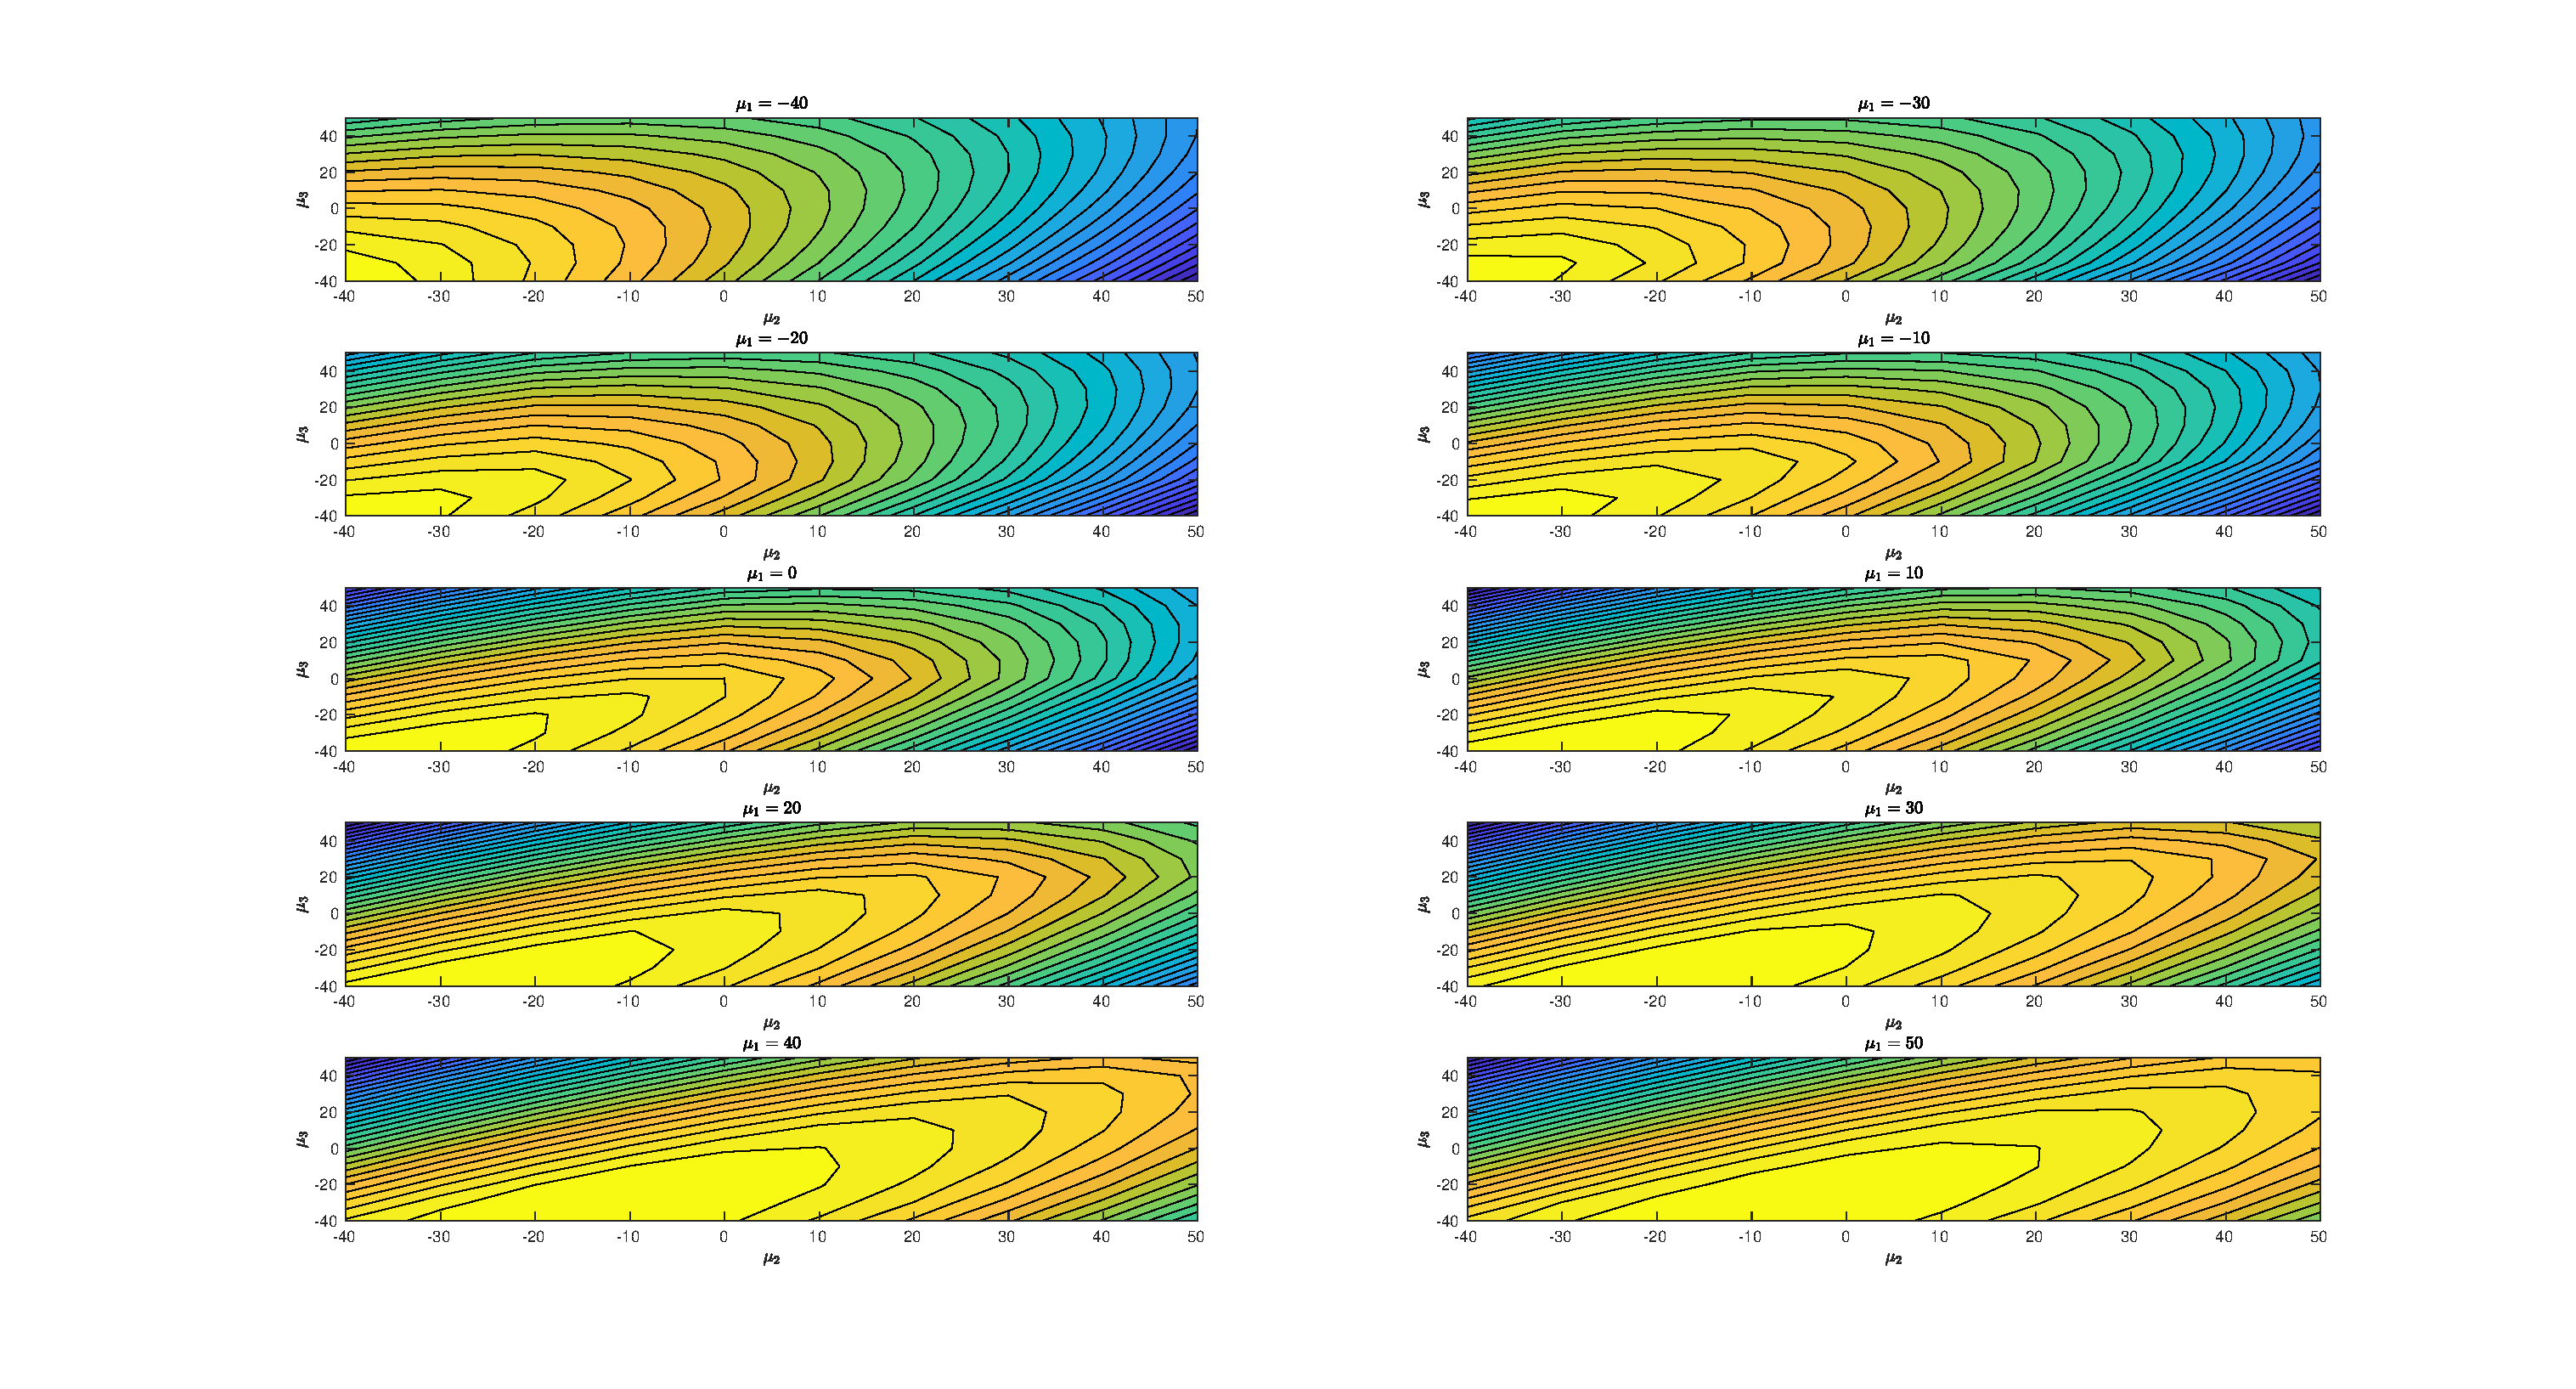
\includegraphics[width=\textwidth]{elbo_contour_plots}
\end{figure*}

\section{Conclusions}

\subsection{Future Work}

%\vskip8pt \noindent
%{\bf Acknowledgments.}
%This is optional; it is a location for you to thank people
\bibliographystyle{abbrv}
\bibliography{paper}
\end{document}